\documentclass[sigconf]{acmart}

%% Remove ACM reference/copyright blocks for course submission
\setcopyright{none}
\acmConference{CSC2524H}{2026}{University of Toronto}
\acmDOI{}
\acmISBN{}
\settopmatter{printacmref=false}

%% Packages
\usepackage{graphicx}
\usepackage{booktabs}
\usepackage{microtype}
\usepackage{subcaption}
\usepackage{caption}
\captionsetup{font=small}

%% ============================================================
%%  TITLE & AUTHORS
%% ============================================================
\title{PromptPaint: Implementation and Extensions}

\author{Thomas Nguyen}
\affiliation{%
  \institution{University of Toronto, Canada}
}
\email{tomasdfgh.nguyen@mail.utoronto.ca}

%% ============================================================
%%  ABSTRACT
%% ============================================================
\begin{abstract}
Text-to-image (T2I) diffusion models make high-quality image generation
accessible, but steering generation toward a specific creative vision remains
difficult. I implement and extend PromptPaint~\cite{chung2023promptpaint},
a tool that applies paint-medium-like interactions to T2I generation, allowing
users to mix prompts, paint spatial regions, and intervene mid-generation.
Beyond re-implementing the original system, I introduce five extensions:
upgrading the backbone to Stable Diffusion XL, supporting an arbitrary number
of mixed prompts, geometrically correct prompt interpolation via Fréchet mean,
post-hoc generation scrubbing, and a multi-user deployment architecture.
I reflect on design trade-offs and discuss directions for future work.
\end{abstract}

\begin{CCSXML}
<ccs2012>
  <concept>
    <concept_id>10003120.10003121.10003122</concept_id>
    <concept_desc>Human-centered computing~Interactive systems and tools</concept_desc>
    <concept_significance>500</concept_significance>
  </concept>
  <concept>
    <concept_id>10010405.10010469</concept_id>
    <concept_desc>Applied computing~Arts and humanities</concept_desc>
    <concept_significance>300</concept_significance>
  </concept>
  <concept>
    <concept_id>10010147.10010178</concept_id>
    <concept_desc>Computing methodologies~Computer vision</concept_desc>
    <concept_significance>300</concept_significance>
  </concept>
</ccs2012>
\end{CCSXML}

\ccsdesc[500]{Human-centered computing~Interactive systems and tools}
\ccsdesc[300]{Applied computing~Arts and humanities}
\ccsdesc[300]{Computing methodologies~Computer vision}

\keywords{generative model, text-to-image generation, painting interactions, diffusion models, prompt mixing}

\begin{document}
\maketitle

%% ============================================================
\section{Introduction}
%% ============================================================

Diffusion-based text-to-image (T2I) models have made high-quality image generation
accessible to non-expert users~\cite{ramesh2022hierarchical,rombach2022high}.
However, prompting remains fundamentally limited as an interaction modality.
Natural language cannot easily express continuous visual attributes, and the
end-to-end nature of most T2I systems leaves users little room to intervene
once generation has begun.

Artists working with physical media do not commit to a final image in one step.
They iterate, layer paint, and make fine-grained decisions throughout the
creation process. Chung and Adar~\cite{chung2023promptpaint} proposed
PromptPaint, which brings this iterative, paint-like workflow to T2I generation
by treating prompts as paint colors that can be mixed, spatially applied, and
changed during diffusion.

In this project, I implement and extend PromptPaint as a full-stack web
application. My contributions are:

\begin{itemize}
  \item \textbf{Model upgrade to SDXL}: replacing the original Stable Diffusion
        v1.5 backbone with Stable Diffusion XL~\cite{podell2023sdxl}, raising
        output resolution from 512$\times$512 to up to 1024$\times$1024 with
        support for nine aspect ratios (1:1, 4:3, 3:2, 16:9, and 21:9 in both
        landscape and portrait) and significantly improved image quality.
  \item \textbf{Arbitrary prompt mixing}: lifting the original three-prompt cap
        to support any number of simultaneously mixed prompts.
  \item \textbf{Fréchet mean interpolation}: replacing linear embedding
        interpolation with the Riemannian center of mass on the CLIP hypersphere,
        producing geometrically correct blends regardless of the number of prompts.
  \item \textbf{Post-hoc generation scrubbing}: all intermediate latents are saved,
        allowing users to branch from any diffusion step after viewing decoded previews,
        removing the timing pressure of live intervention.
  \item \textbf{Publicly accessible web deployment}: an always-available web
        application backed by a GPU job queue, session isolation, and per-IP
        rate limiting, making PromptPaint accessible to anyone without local
        setup.
\end{itemize}

\begin{figure*}[!t]
  \centering
  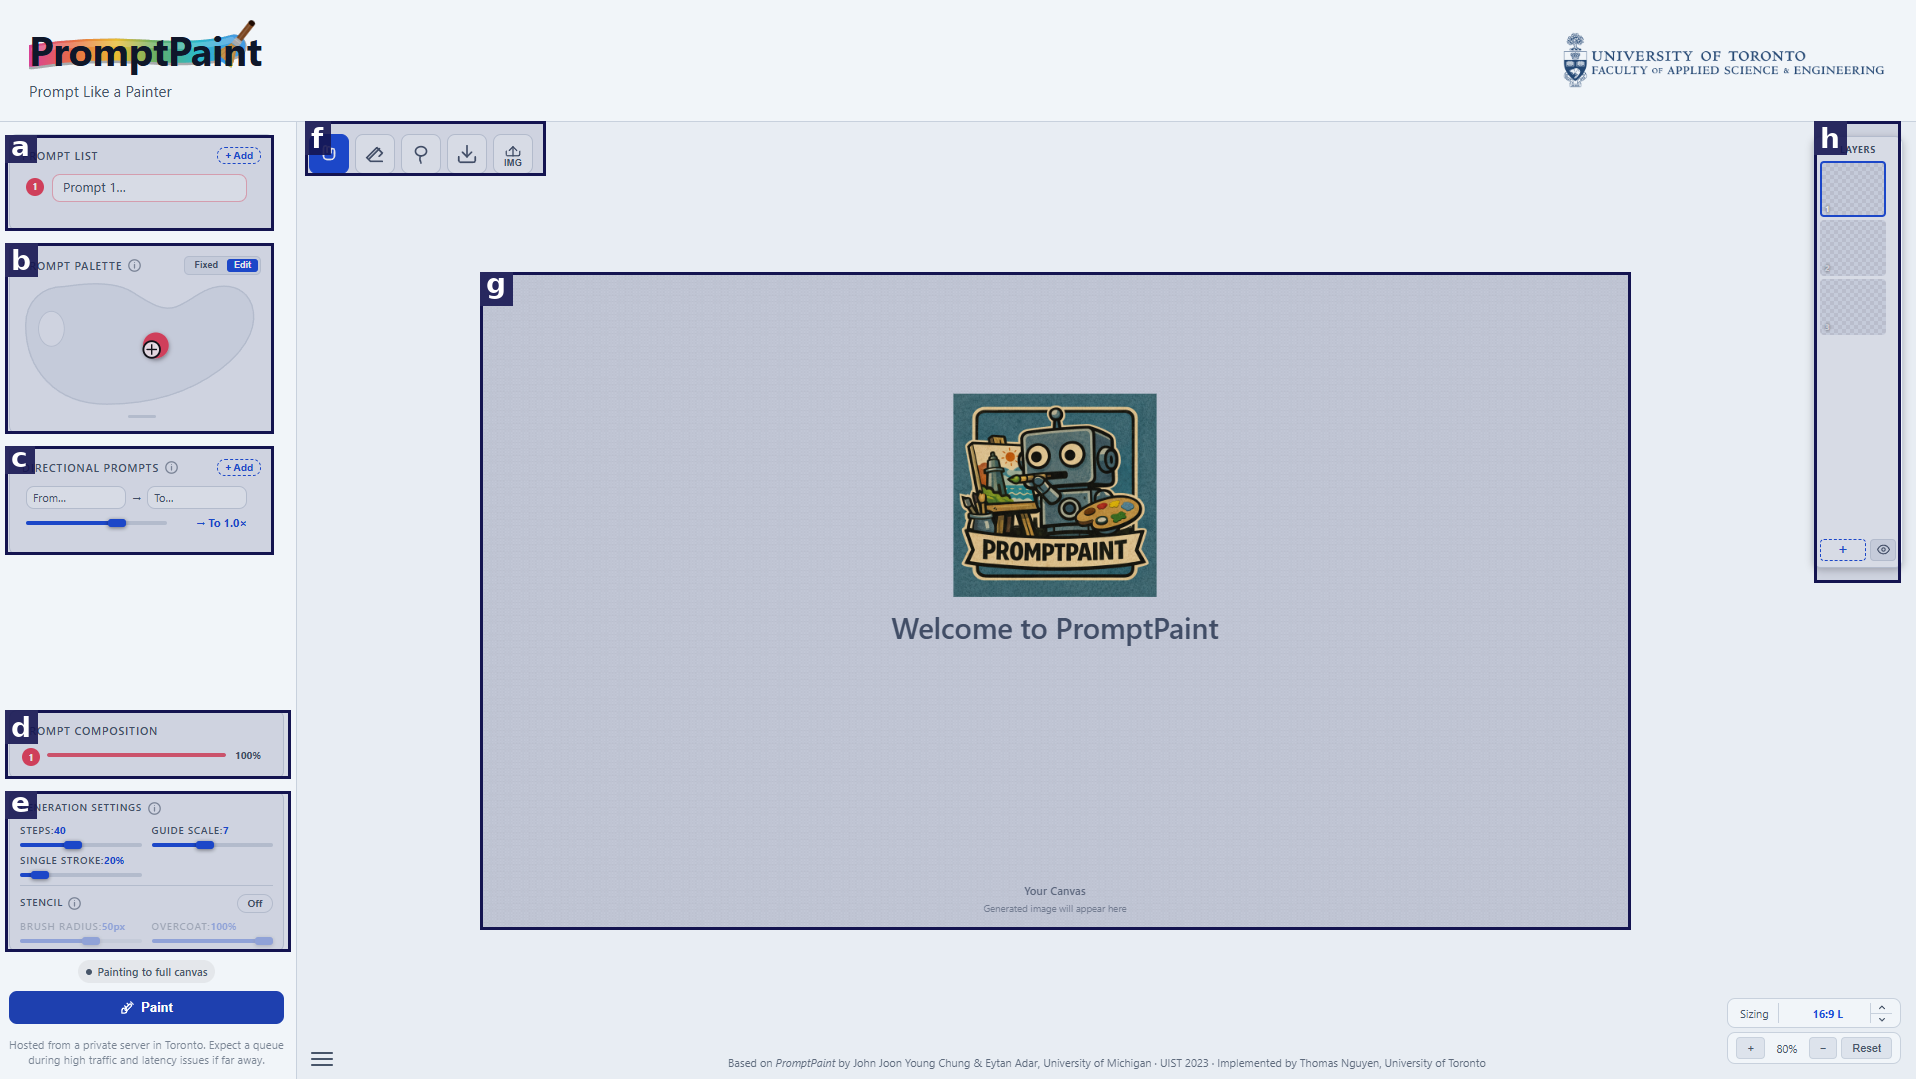
\includegraphics[width=\linewidth]{ui_layout_labeled}
  \caption{The PromptPaint interface. (a)~Prompt List: active prompts whose
  embeddings are blended on the palette. (b)~Prompt Palette: prompt nodes
  can be dragged to reposition and blend them; a cursor sets per-prompt
  weights by proximity, mixing their embeddings via Fréchet mean interpolation. (c)~Directional Prompts: ``from'' and
  ``to'' concept endpoints with a scalar weight that shifts the mixed
  embedding along a semantic direction. (d)~Prompt Composition: real-time
  readout of per-prompt weight contributions. (e)~Generation Settings:
  controls for diffusion steps, guidance scale, single-stroke brush size,
  stencil mode, brush radius, and overcoat ratio; revealed by hovering over
  the Paint button. (f)~Toolbar: mode selector for generate, erase, lasso,
  export, and image upload. (g)~Canvas: the main drawing surface; brush
  strokes define the stencil region for spatially targeted generation.
  (h)~Layers: layer stack with per-layer opacity and visibility controls.}
  \label{fig:ui}
\end{figure*}

%% ============================================================
\section{Background and Related Work}
%% ============================================================

\subsection{Diffusion-based Text-to-Image Generation}

Latent diffusion models~\cite{rombach2022high} generate images by iteratively
denoising a latent representation guided by a text encoder (CLIP~\cite{radford2021learning}).
The denoising process runs for $K$ steps (configurable by the user), with
earlier steps establishing global structure and later steps refining detail.
Because the process is Markovian, each step depends only on the current
latent and not on the full history of how it got there, so it is possible
to branch at any step by substituting a saved latent and continuing
denoising with a different prompt. This temporal structure makes the generation process a
natural target for interactive intervention.

\subsection{Prompt Engineering}

Despite their power, T2I models place a significant burden on users to craft
effective prompts. Liu and Chilton~\cite{liu2022promptengineering} conducted a
systematic study of prompt engineering strategies for T2I models, finding that
subject, style, and attribute descriptors each interact differently with model
outputs. Subtle wording changes can produce dramatically different results,
making the relationship between language and image opaque to users.
Their design guidelines highlight that natural language alone is often
insufficient for expressing precise visual intent, motivating interaction
approaches that go beyond raw text entry. PromptPaint directly addresses
this by letting users explore the semantic space between prompts visually
rather than through iterative text revision.

\subsection{Steering Generative Models}

Prior work has explored steering T2I generation through sliders~\cite{gandissect},
examples~\cite{gal2022image}, and prompt editing~\cite{brooks2023instructpix2pix}.
Mixing approaches have combined two prompts via linear interpolation of
embeddings~\cite{liu2022compositional} or by combining them textually.
These methods typically operate on pairs of concepts and do not account for
the geometry of the high-dimensional embedding space.
PromptPaint~\cite{chung2023promptpaint} unified these approaches under a
paint-medium metaphor and identified four distinct interaction strategies,
characterizing their trade-offs through a crowdsourced study.

\subsection{Image Editing and Inpainting}

Several approaches enable spatially targeted image editing with diffusion models.
Blended Diffusion~\cite{avrahami2022blended} composites text-guided diffusion
within user-defined masked regions, blending the generated content with the
surrounding image in latent space. SDEdit~\cite{meng2021sdedit} adds noise to
an existing image and denoises it with a new prompt, providing a controllable
trade-off between faithfulness to the original and adherence to the new
prompt. Both methods highlight the role of the noise schedule in mediating
between preservation and change. The prompt stencil mechanism in PromptPaint
draws on similar principles, using the overcoat parameter to directly expose
this trade-off to the user.

\subsection{Interactive Control During Generation}

Prompt2Prompt~\cite{hertz2022prompt} demonstrated that cross-attention maps
can be manipulated mid-generation for fine-grained edits, enabling targeted
changes to specific objects without affecting the rest of the image.
ControlNet~\cite{zhang2023adding} enables structural conditioning at generation
time via auxiliary inputs such as depth maps or edge maps. These methods expose
powerful low-level controls but require users to reason about attention weights
or provide structured auxiliary inputs. This work complements them by focusing
on the \emph{interaction design} layer: how users can intuitively steer
generation through paint-like affordances without requiring technical knowledge
of model internals.

\subsection{Human-AI Creative Co-creation}

Beyond image generation, researchers have explored how AI can be integrated
into broader creative workflows. TaleBrush~\cite{chung2022talebrush} demonstrates
how sketch-based interactions can guide generative language models to produce
narratives, showing that paint-like affordances extend naturally to other
generative modalities. This line of work motivates the design principle behind
PromptPaint: that creative AI tools should support the iterative, incremental
workflows of human artistic practice rather than reducing creation to a
single prompt-and-result interaction.

%% ============================================================
\section{System Design}
%% ============================================================

PromptPaint is a three-tier web application: a React frontend, a Flask+Socket.IO
backend, and a FastAPI model service running SDXL on a dedicated GPU. The
separation of model and backend services allows the backend to be restarted
independently without reloading the model weights from disk. The system
implements all four interaction modes from the original paper (prompt mixing,
prompt stencil, directional prompts, and prompt intervention) and extends
two of them as described below.

\subsection{Prompt Mixing via Fréchet Mean}

As in the original paper~\cite{chung2023promptpaint}, users position a cursor
on a visual palette to blend any number of text prompts simultaneously. The
palette maps cursor position to per-prompt weights $w_i$, and the weighted
embeddings are combined into a single mixed prompt passed to the denoiser.
The original system interpolates embeddings linearly:

\begin{equation}
  v_{m} = \sum_{i=1}^{N} w_i \, v_i
\end{equation}

Linear interpolation in high-dimensional space cuts through the interior of
the CLIP hypersphere, producing undersized vectors that are out-of-distribution
for the text encoder. The original paper supports up to three prompts; I
generalize this to an arbitrary number and replace the linear blend with the
\textbf{Fréchet mean}~\cite{frechet1948elements}, the Riemannian center of mass
on the unit hypersphere, computed iteratively via the exponential and logarithmic maps:

\begin{equation}
  \mu_{t+1} = \exp_{\mu_t}\!\left(\sum_{i=1}^{N} w_i \log_{\mu_t}(v_i)\right)
\end{equation}

This ensures the mixed embedding remains on the hypersphere regardless of the
number of prompts or their angular separation, producing more semantically coherent
blends especially at SDXL's 2048-dimensional embedding scale.

\begin{figure}[t]
  \centering
  \begin{subfigure}{\linewidth}
    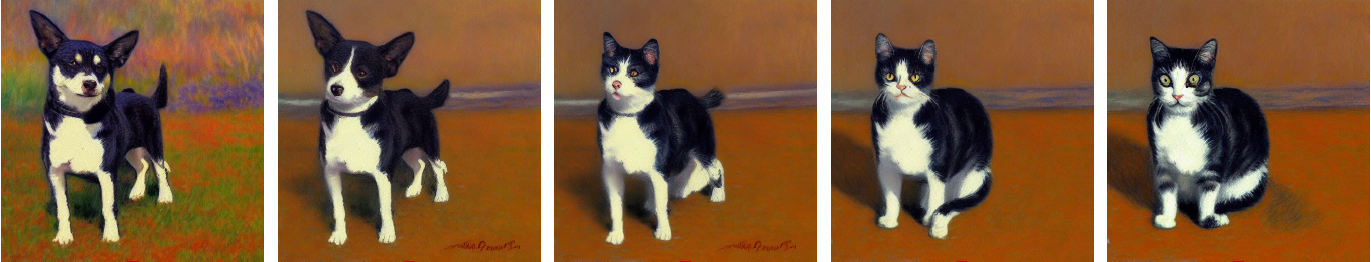
\includegraphics[width=\linewidth]{paper_dog_to_cat}
    \caption*{\textit{Original paper} (Chung \& Adar, 2023): linear interpolation,
    SD\,v1.5, 512$\times$512}
  \end{subfigure}
  \vspace{2pt}
  \begin{subfigure}{\linewidth}
    
\includegraphics[width=\linewidth]{fig_prompt_mixing}
    \caption*{\textit{This work}: Fréchet mean interpolation, SDXL, 1024$\times$1024}
  \end{subfigure}
  \caption{Prompt mixing between ``a dog'' and ``a cat'' at five evenly spaced
  weights. Top: original paper using linear embedding interpolation on SD\,v1.5.
  Bottom: our Fréchet mean interpolation on SDXL, which keeps the mixed embedding
  on the CLIP hypersphere for more coherent blends.}
  \label{fig:prompt_mixing}
\end{figure}

\begin{figure}[h]
  \centering
  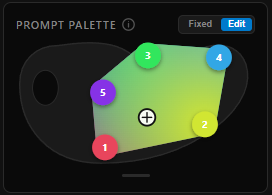
\includegraphics[width=0.75\linewidth]{more_than_3_prompt_mixed}
  \caption{The prompt palette with five simultaneous prompts. Each numbered
  node represents a distinct text prompt; the crosshair position determines the
  per-prompt weights via Fréchet mean interpolation. The original paper
  supported at most three prompts.}
  \label{fig:five_prompts}
\end{figure}

\subsection{Prompt Stencil}

Following~\cite{chung2023promptpaint}, users paint a region on the canvas
with a brush to spatially constrain where generation occurs. The brush strokes
are converted to a binary mask $M$ in latent space (at $1/8$ the pixel
resolution). During denoising, for steps $k < (1 - o/100) \cdot K$ (where
$o$ is the overcoat ratio), the painted region is reset to the noisy version
of the original image latent, anchoring the stenciled area to the existing
canvas. For later steps, the mask is applied as:

\begin{equation}
  z_{m,k} = M \odot z_k + (1 - M) \odot v(z_I, k)
\end{equation}

where $z_I$ is the encoded original image latent and $v(\cdot, k)$ adds
scheduler-appropriate noise for step $k$. This matches equations~(4--5)
of~\cite{chung2023promptpaint}.

\subsection{Directional Prompts}

Following~\cite{chung2023promptpaint}, a directional prompt is defined by two
concept endpoints $c_1$ (``from'') and $c_2$ (``to'') with a scalar weight
$w_d$. The directional vector $v_d = v_{c_2} - v_{c_1}$ is added to the
mixed prompt embedding:

\begin{equation}
  v_f = v_m + \sum_{j=1}^{M} w_{d_j} \, v_{d_j}
\end{equation}

where $v_m$ is the mixed prompt embedding from Section~3.1. Each weight $w_{d_j}$ is exposed to the user as a dial beneath its corresponding directional prompt pair in the interface, allowing fine-grained attribute control (e.g., matte $\to$ glossy) without rewriting the base prompt. Multiple directional prompts can be stacked.

\begin{figure}[h]
  \centering
  
\includegraphics[width=\linewidth]{fig_directional}
  \caption{Directional prompt: shifting from ``young'' to ``old'' at five
  evenly spaced weight values, holding the base prompt constant.}
  \label{fig:directional}
\end{figure}

\begin{figure}[h]
  \centering
  \begin{subfigure}{\linewidth}
    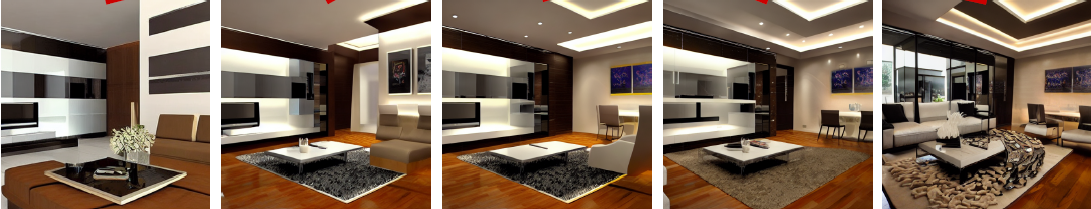
\includegraphics[width=\linewidth]{paper_simple_to_complex_interior_home_design}
    \caption*{\textit{Original paper} (Chung \& Adar, 2023): live directional
    prompt applied during generation}
  \end{subfigure}
  \vspace{2pt}
  \begin{subfigure}{\linewidth}
    
\includegraphics[width=\linewidth]{simple_to_complex_gradient}
    \caption*{\textit{This work}: directional prompt on SDXL}
  \end{subfigure}
  \caption{Directional prompt applied to ``interior home design,'' shifting
  from ``simple'' to ``complex'' at five evenly spaced weight values. The
  scene progressively gains architectural detail, layered furnishings, and
  visual density while the base prompt remains unchanged.}
  \label{fig:directional_interior}
\end{figure}

\subsection{Prompt Intervention}

Prompt intervention allows users to branch a generation mid-way by switching
to a new prompt at a chosen diffusion step $k^*$. Because the DDPM denoising
process is Markovian, the latent $z_{k^*}$ encodes the structural information
committed so far (global composition, rough shapes) while leaving later steps
free to respond to a new prompt. The result is a generated image that blends
the compositional intent of the original prompt with the semantic content of
the new one: earlier branch points favour the new prompt; later ones preserve
more of the original structure.

\begin{figure}[h]
  \centering
  \begin{subfigure}{\linewidth}
    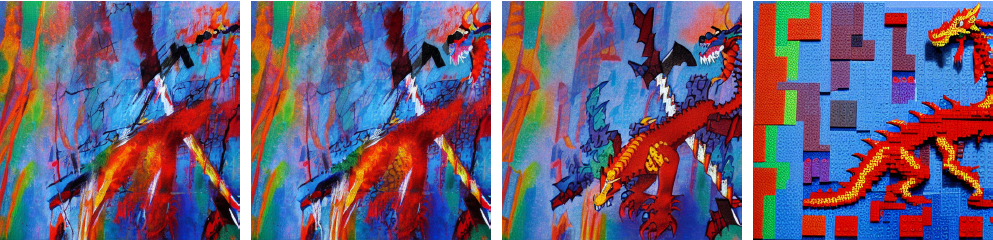
\includegraphics[width=\linewidth]{dragon_to_lego_paper}
    \caption*{\textit{Original paper} (Chung \& Adar, 2023): live prompt
    intervention during generation}
  \end{subfigure}
  \vspace{2pt}
  \begin{subfigure}{\linewidth}
    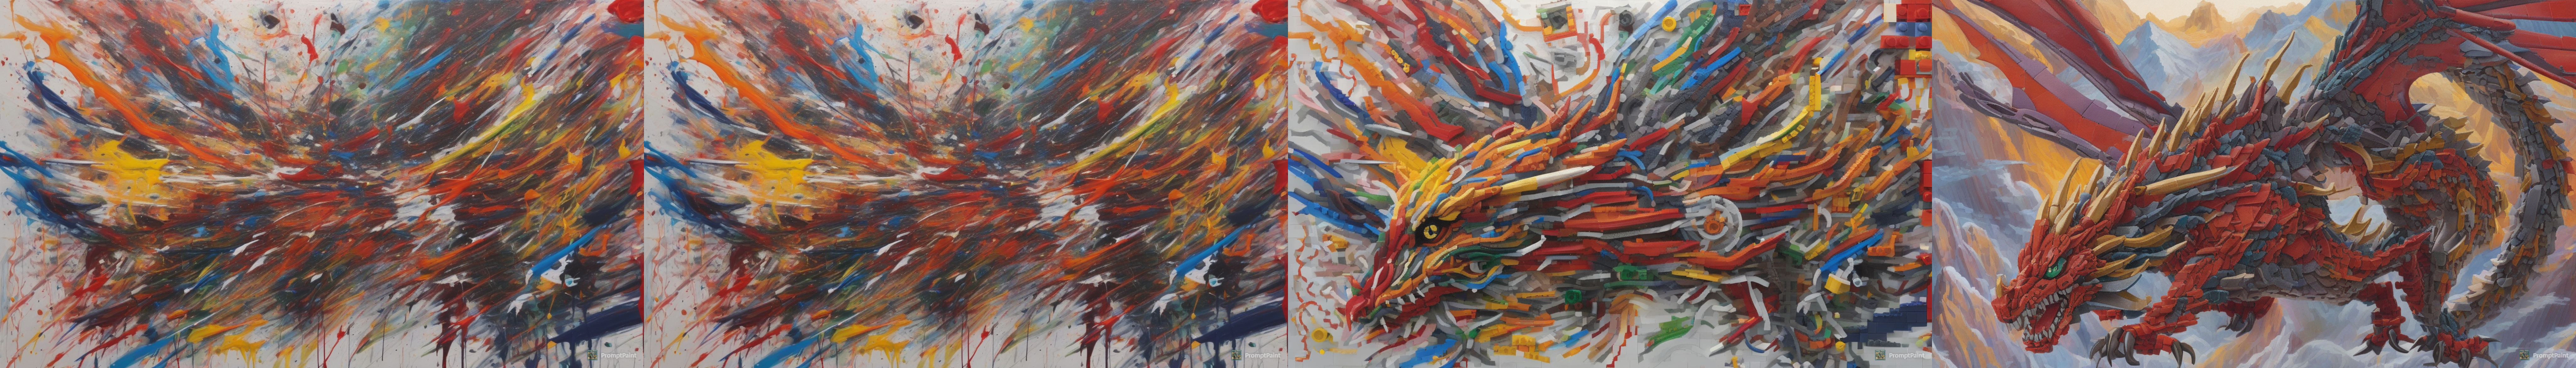
\includegraphics[width=\linewidth]{fig_scrubbing_result}
    \caption*{\textit{This work}: post-hoc scrubbing from saved latents}
  \end{subfigure}
  \caption{Prompt intervention during generation. Top: original paper's live
  dragging interaction, branching from ``action painting'' mid-generation.
  Bottom: our post-hoc scrubbing approach, where the user selects a branch
  point after viewing decoded step previews, then resumes with a new prompt
  (here, ``a dragon'') from the saved latent.}
  \label{fig:scrubbing_result}
\end{figure}

\begin{figure}[h]
  \centering
  \begin{subfigure}{\linewidth}
    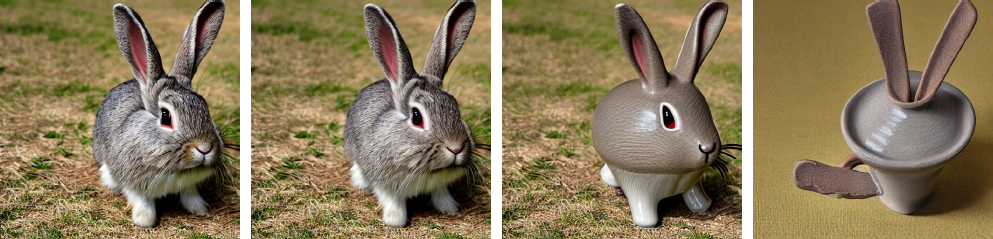
\includegraphics[width=\linewidth]{rabbit_to_ceramic_cup_paper}
    \caption*{\textit{Original paper} (Chung \& Adar, 2023): live prompt
    intervention during generation}
  \end{subfigure}
  \vspace{2pt}
  \begin{subfigure}{\linewidth}
    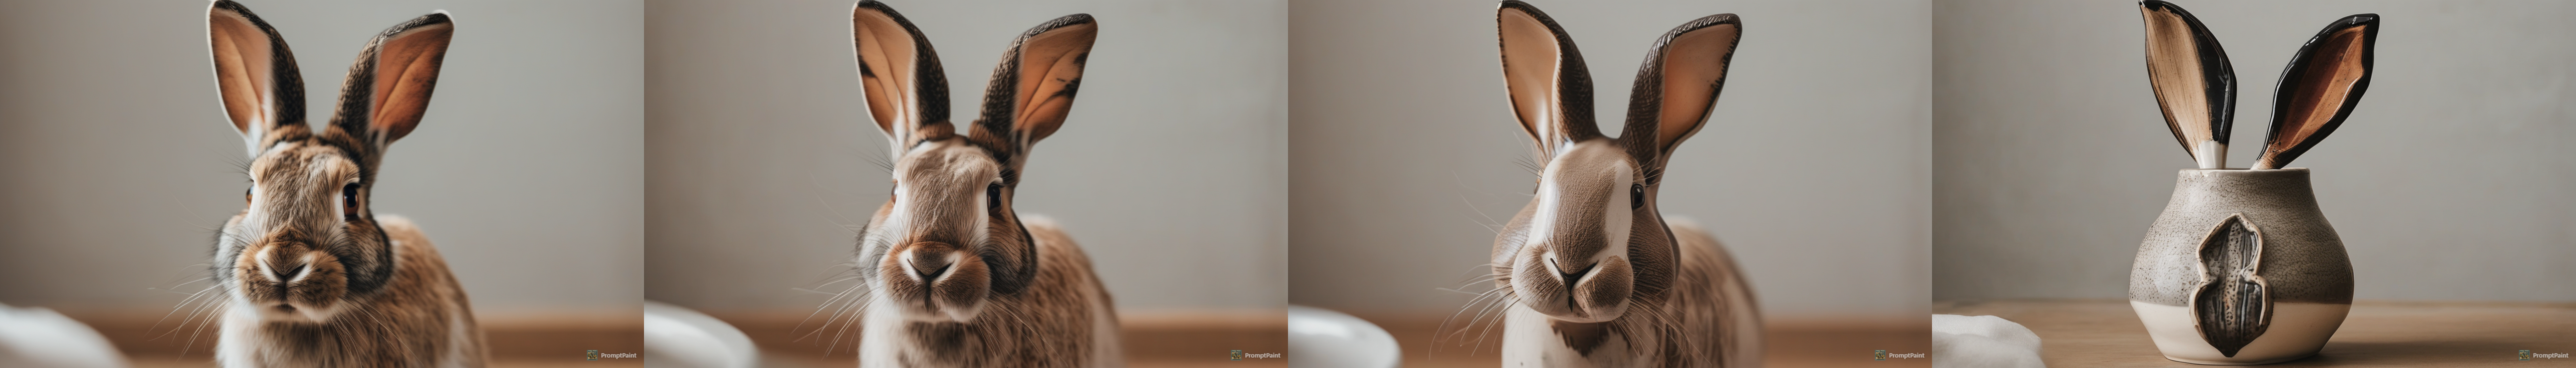
\includegraphics[width=\linewidth]{fig_rabbit_ceramic}
    \caption*{\textit{This work}: post-hoc scrubbing from saved latents}
  \end{subfigure}
  \caption{Prompt intervention switching from ``a rabbit'' to ``a ceramic vase.''
  Top: original paper's live dragging approach. Bottom: our post-hoc scrubbing,
  where the user branches from a saved intermediate latent. Earlier steps
  preserve the subject's form; later steps resolve the new material and shape.}
  \label{fig:intervention}
\end{figure}

\subsection{Post-hoc Generation Scrubbing}

The original system requires users to change prompts \emph{during} an ongoing
generation, which demands precise timing and offers no visual feedback on
intermediate states. The original paper's own user study found this to be the
hardest interaction to use~\cite{chung2023promptpaint}.

I replace live intervention with \textbf{post-hoc scrubbing}: at each
diffusion step $k$, the intermediate latent $z_k$ is saved to CPU memory.
After generation completes, users scrub through a step-by-step preview bar,
select a branch point, update the prompt palette, and resume generation from
the saved $z_{k^*}$, skipping timesteps $[0, k^*)$ and denoising only the
remaining steps with the new embedding. This is mathematically equivalent to
live intervention (same Markov branch point) but removes all timing pressure
and gives users decoded visual previews before committing to a branch.

\subsection{Model Selection}

The original PromptPaint paper used Stable Diffusion v1.5~\cite{rombach2022high},
a latent diffusion model operating at 512$\times$512 resolution with 768-dimensional
CLIP text embeddings. I upgrade the backbone to Stable Diffusion XL
(SDXL)~\cite{podell2023sdxl}, which operates at up to 1024$\times$1024 native
resolution with a dual text encoder producing 2048-dimensional embeddings.
The larger embedding space provides finer semantic granularity for prompt mixing
and directional shifts, and the higher resolution yields significantly more
detailed outputs, both properties that directly benefit the paint-medium
interactions this system is built around.

A stronger model (e.g., a fine-tuned SDXL variant or a newer architecture)
could in principle improve output quality further. However, the system is
designed as a publicly accessible, always-on web deployment, and the choice
of model is therefore constrained by VRAM budget on the host machine (two
NVIDIA A4000 GPUs, 16\,GB each, 32\,GB total). SDXL in float16 occupies
approximately 8\,GB of VRAM (roughly 25\% of total capacity), leaving
the remaining VRAM available for other workloads on the same machine while
keeping the model permanently loaded without cold-start latency for users.
This balance between model capability and resource footprint guided the
final selection.

\begin{figure}[h]
  \centering
  \begin{subfigure}{0.75\linewidth}
    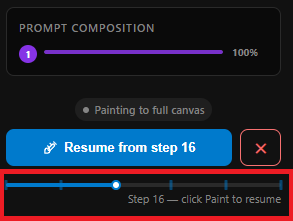
\includegraphics[width=\linewidth]{scrubber}
    \caption*{After generation completes, the user drags the scrub bar to any
    saved diffusion step, repositions the palette crosshair to a different
    prompt mix, and clicks \emph{Resume} to continue denoising from that
    latent, with no timing pressure required.}
  \end{subfigure}
  \vspace{4pt}
  \begin{subfigure}{0.75\linewidth}
    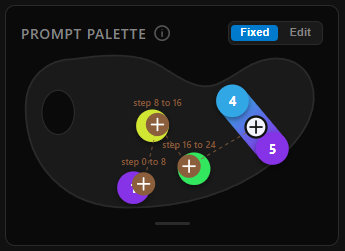
\includegraphics[width=\linewidth]{generation_timeline}
    \caption*{The prompt palette overlays a generation timeline, annotating
    which prompt mix was active during each step interval so the user can
    trace how the image evolved and choose an informed branch point.}
  \end{subfigure}
  \caption{Post-hoc scrubbing workflow.}
  \label{fig:scrubber}
\end{figure}

%% ============================================================
\section{Implementation}
%% ============================================================

\subsection{Technology Stack}

The model service runs SDXL (\texttt{stabilityai/\allowbreak stable-diffusion-xl-\allowbreak base-1.0})
with a CLIP ViT-L/14 text encoder, Euler Discrete scheduler, and float16
precision (float32 VAE). All prompt manipulations occur in the text
embedding space before the UNet denoiser, consistent with the approach
taken in the original paper~\cite{chung2023promptpaint}. The system is containerized with
Docker Compose and served behind an Nginx reverse proxy.

\subsection{Multi-user Architecture}

The original PromptPaint paper described a research prototype and did not
address multi-user deployment. My implementation extends this to serve
multiple concurrent users over the web.
A single GPU worker thread serializes all generation jobs through a
stdlib \texttt{Queue}, ensuring no VRAM contention. Each user session is
isolated via a session ID, and intermediate latents are keyed by
(session\_id, step). The Flask backend enforces per-IP concurrency limits
(at most one active generation per IP) and cooldown timers to prevent
resource exhaustion. The system is publicly accessible at
\url{https://promptpaint.tom-nguyen.ca}. Source code is available at
\url{https://github.com/Tomasdfgh/PromptPaint}, and a demo video is available at
\url{https://www.youtube.com/watch?v=Ws-_sAdnccU}.

\subsection{Streaming Previews}

Generation results are streamed to the frontend via Socket.IO as
newline-delimited JSON events. Each diffusion step emits a \texttt{progress}
event with a base64-encoded preview image decoded from the current latent,
giving users real-time visual feedback throughout the denoising process.

%% ============================================================
\section{Discussion}
%% ============================================================

\subsection{Design Trade-offs}

My implementation surfaces several trade-offs identified in the
original paper~\cite{chung2023promptpaint}. The post-hoc scrubbing approach
resolves the timing difficulty of live prompt intervention but changes the
interaction model: users must wait for a full generation before branching,
rather than steering an in-progress generation. This trades immediacy for
informed decision-making, which my informal testing suggests is preferable
for most users.

The Fréchet mean improves semantic coherence for mixed prompts but introduces
a small computational overhead ($\sim$5 iterations of the iterative solver
per generation request); however, this is negligible compared to UNet inference time.

\subsection{Limitations}

The system currently has no negative prompt interface, limiting the user's
ability to suppress unwanted content. The stencil interaction can produce
style inconsistencies at region boundaries, particularly at high overcoat
values. The multi-user architecture does not persist latents across server
restarts, so scrubbing state is lost if the model service is restarted.

\subsection{Future Work}

Several directions could extend this work. First, making intermediate
latent representations more interpretable (for example, using progressive
denoising visualizations~\cite{ho2020denoising}) would lower the learning
curve for prompt intervention. Second, incorporating structural conditioning
(e.g., ControlNet~\cite{zhang2023adding}) into the stencil interaction
would allow users to constrain generation with sketch or depth inputs.
Third, and most importantly for evaluation, a longitudinal user study
comparing post-hoc scrubbing to live intervention would be the first
experiment worth running: the scrubber is the most novel interaction in
this system and the one whose benefit is hardest to demonstrate without
empirical data. The original paper's user study already identified live
intervention as the hardest interaction to use~\cite{chung2023promptpaint},
making a direct comparison a natural and well-motivated first study. Finally, the Fréchet mean framework could be extended
to image exemplar embeddings, enabling users to mix image references
alongside text prompts on the same palette.

%% ============================================================
\section{Conclusion}
%% ============================================================

I implemented and extended PromptPaint as a full-stack web application.
My extensions, including an SDXL backbone, Fréchet mean prompt mixing for arbitrary
numbers of prompts, post-hoc generation scrubbing, and a publicly accessible
deployment, build on the original research prototype while preserving the core
paint-medium interaction metaphor. The implementation demonstrates that diffusion model internals
(embedding geometry, intermediate latents, denoising schedules) can be
exposed to users through intuitive, paint-inspired affordances, supporting
both focused iteration and open-ended creative exploration.

%% ============================================================
%%  REFERENCES
%% ============================================================
\clearpage
\bibliographystyle{ACM-Reference-Format}
\bibliography{references}

\end{document}
